\chapter{कार्बनिक अणु: कंकाल और नाम}\label{ch:g11:organic-skeletons}

एक बार इस्तेमाल होने वाले लाइटर में ब्यूटेन होती है, दाब के कारण द्रव; बर्फ़ीले पहाड़
पर ले जाए गए कैंपिंग स्टोव के कारतूस में प्रोपेन होती है, या उससे अधिक समृद्ध कोई
\omterm{def:g6:pure-substances-and-mixtures:mixture}{मिश्रण}। दोनों केवल कार्बन और हाइड्रोजन \omterm{def:g7:atoms-and-molecules:atom}{परमाणुओं} से बने हैं,
और दोनों एक विशाल परिवार के हैं: कार्बन \omterm{def:g7:atoms-and-molecules:atom}{परमाणुओं} के कंकाल पर बने \omterm{def:g7:atoms-and-molecules:molecule}{अणु}। ऐसे लाखों
\omterm{def:g7:atoms-and-molecules:molecule}{अणु} ज्ञात हैं। उनके बारे में बात करने के लिए रसायनज्ञों को उन्हें जल्दी से बनाने और
बिना किसी अस्पष्टता के उनके नाम रखने के तरीके चाहिए।

\begin{recall}
कार्बन चार \omterm{def:g10:lewis-and-shape:covalent-bond}{सहसंयोजी आबंध} बनाता है और हाइड्रोजन एक; चार एकल आबंधों वाले कार्बन
\omterm{def:g7:atoms-and-molecules:atom}{परमाणु} के चारों ओर आबंध एक चतुष्फलक के कोनों की ओर इशारा करते हैं,
लगभग \ang{109.5} पर (\cref{ch:g10:lewis-and-shape})।
\end{recall}

\begin{omfigure}
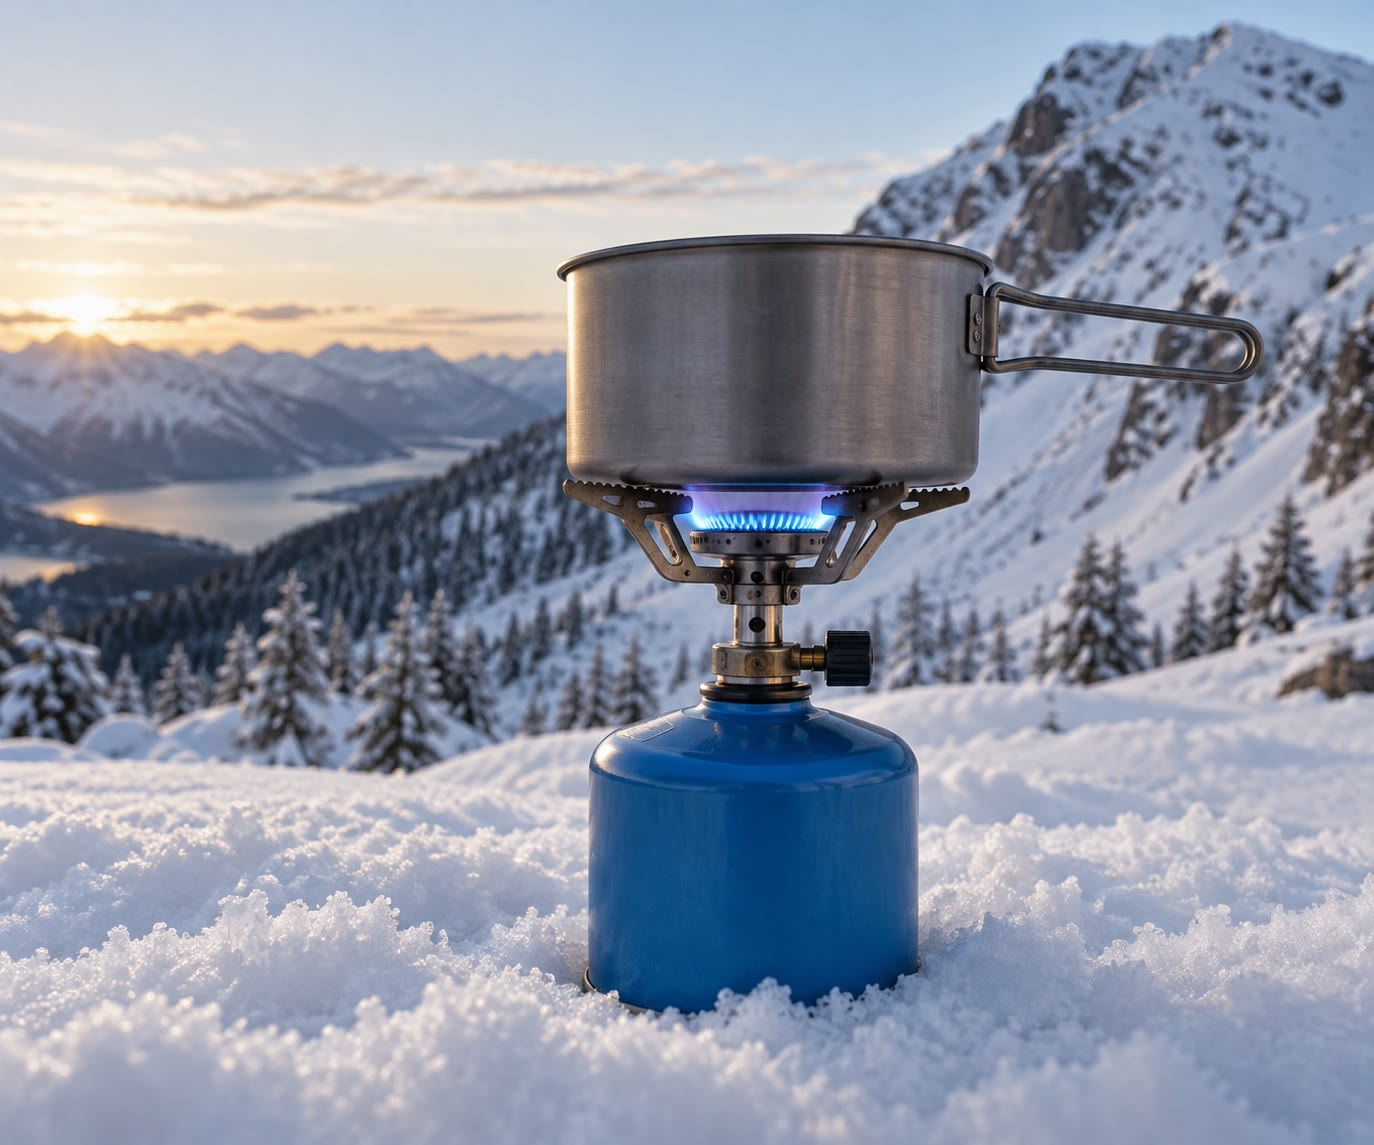
\includegraphics[width=0.48\linewidth]{images/book1/ai/g11-camping-cartridge.jpg}

{\small बर्फ़ में एक कैंपिंग स्टोव, जो कार्बन और हाइड्रोजन से बनी एक गैस
जला रहा है।}
\end{omfigure}

\section{कार्बनिक अणुओं के सूत्र}

\begin{definition}[कार्बनिक यौगिक]\label{def:g11:organic-skeletons:organic}
\emph{कार्बनिक यौगिक}\index{कार्बनिक यौगिक} वह यौगिक है जिसके
\omterm{def:g7:atoms-and-molecules:molecule}{अणु} एक-दूसरे से और हाइड्रोजन \omterm{def:g7:atoms-and-molecules:atom}{परमाणुओं} से आबंधित कार्बन \omterm{def:g7:atoms-and-molecules:atom}{परमाणुओं} के कंकाल पर बने
होते हैं, संभवतः ऑक्सीजन और नाइट्रोजन जैसे दूसरे \omterm{def:g7:atoms-and-molecules:atom}{परमाणुओं} के साथ।
(कार्बन डाइऑक्साइड, कार्बन मोनोऑक्साइड और कार्बोनेटों को परंपरागत रूप से
इसमें नहीं गिना जाता।)
\end{definition}

\begin{definition}[सूत्र के चार प्रकार]\label{def:g11:organic-skeletons:formulas}
किसी \omterm{def:g7:atoms-and-molecules:molecule}{अणु} को चार तरह से लिखा जा सकता है:
\begin{itemize}
  \item उसका \emph{आण्विक सूत्र}\index{आण्विक सूत्र} केवल हर तत्व के
        \omterm{def:g7:atoms-and-molecules:atom}{परमाणुओं} की संख्या देता है, जैसे \ce{C4H10};
  \item उसका \emph{संरचना सूत्र}\index{संरचना सूत्र} हर \omterm{def:g7:atoms-and-molecules:atom}{परमाणु}
        और हर आबंध दिखाता है;
  \item उसका \emph{अर्ध-संरचना सूत्र}\index{अर्ध-संरचना सूत्र}
        कार्बन \omterm{def:g7:atoms-and-molecules:atom}{परमाणुओं} के बीच के आबंध दिखाता है और हाइड्रोजन \omterm{def:g7:atoms-and-molecules:atom}{परमाणुओं} को उनके
        कार्बन के साथ समूहित करता है, जैसे \ce{CH3-CH2-CH2-CH3};
  \item उसका \emph{कंकाल सूत्र}\index{कंकाल सूत्र} केवल कार्बन कंकाल के
        आबंधों को टेढ़ी-मेढ़ी रेखा के रूप में बनाता है: हर सिरा और हर
        कोना एक कार्बन \omterm{def:g7:atoms-and-molecules:atom}{परमाणु} है, कार्बन पर लगे हाइड्रोजन \omterm{def:g7:atoms-and-molecules:atom}{परमाणु} नहीं
        बनाए जाते, और हर दूसरा \omterm{def:g7:atoms-and-molecules:atom}{परमाणु} (अपने हाइड्रोजन \omterm{def:g7:atoms-and-molecules:atom}{परमाणुओं} के साथ) लिखा जाता है।
\end{itemize}
\end{definition}

\begin{omfigure}
\setchemfig{atom sep=1.45em}
\renewcommand{\arraystretch}{1.6}
\small
\begin{tabular}{@{}l@{\quad}c@{\quad}c@{}}
 & ब्यूटेन & 2-मेथिलप्रोपेन \\
आण्विक & \ce{C4H10} & \ce{C4H10} \\[4pt]
संरचना &
\chemfig{H-C(-[2]H)(-[6]H)-C(-[2]H)(-[6]H)-C(-[2]H)(-[6]H)-C(-[2]H)(-[6]H)-H} &
\chemfig{H-C(-[2]H)(-[6]H)-C(-[6]H)(-[2,1.5]C(-[1]H)(-[3]H)(-[2]H))-C(-[2]H)(-[6]H)-H} \\[10pt]
अर्ध-संरचना & \ce{CH3-CH2-CH2-CH3} &
\chemfig{CH_3-CH(-[6]CH_3)-CH_3} \\[14pt]
कंकाल & \chemfig{-[:30]-[:-30]-[:30]} & \chemfig{-[:30](-[:90])-[:-30]} \\
\end{tabular}

{\small ब्यूटेन और 2-मेथिलप्रोपेन के चारों सूत्र। \omterm{def:g11:organic-skeletons:formulas}{कंकाल सूत्रों} में
रेखाओं का हर सिरा और हर कोना एक कार्बन \omterm{def:g7:atoms-and-molecules:atom}{परमाणु} है:
हर एक में चार।}
\end{omfigure}


\begin{example}[कंकाल सूत्र पढ़ना]\label{ex:g11:organic-skeletons:reading}
ब्यूटेन के \omterm{def:g11:organic-skeletons:formulas}{कंकाल सूत्र} में टेढ़ी-मेढ़ी रेखा के दो सिरे और दो कोने हैं:
चार कार्बन \omterm{def:g7:atoms-and-molecules:atom}{परमाणु}। हर सिरे वाले कार्बन का एक आबंध बना है, इसलिए उस पर
तीन हाइड्रोजन \omterm{def:g7:atoms-and-molecules:atom}{परमाणु} हैं (\ce{CH3}); हर कोने के दो आबंध बने हैं,
इसलिए उस पर दो (\ce{CH2})। हर कार्बन के कुल चार आबंध हैं, जिससे
फिर \ce{C4H10} मिलता है।
\end{example}

\section{कार्बन श्रृंखलाएँ}

किसी \omterm{def:g7:atoms-and-molecules:molecule}{अणु} का कार्बन कंकाल एक \emph{रैखिक} श्रृंखला हो सकता है, जिसमें हर
कार्बन अधिक से अधिक दो दूसरों से आबंधित हो, जैसे ब्यूटेन में; एक \emph{शाखित}
श्रृंखला, जिसमें कम से कम एक कार्बन तीन या चार दूसरों से आबंधित हो, जैसे
2-मेथिलप्रोपेन में; या एक \emph{वलय}, जैसे साइक्लोहेक्सेन, \ce{C6H12}, में, जिसका
\omterm{def:g11:organic-skeletons:formulas}{कंकाल सूत्र} एक षट्भुज है। श्रृंखलाओं के लिए टेढ़ी-मेढ़ी रेखा का उपयोग इसलिए होता है
कि हर कार्बन के चारों ओर वास्तविक आबंध लगभग \ang{109.5} के कोण बनाते हैं,
\ang{180} के नहीं: ``रैखिक'' श्रृंखला वास्तव में त्रिविम में एक टेढ़ी-मेढ़ी रेखा है।

\begin{omfigure}
\setchemfig{atom sep=1.9em}
\begin{tabular}{ccc}
\chemfig{-[:30]-[:-30]-[:30]-[:-30]-[:30]} &
\chemfig{-[:30](-[:90])-[:-30]-[:30](-[:90])-[:-30]} &
\chemfig{*6(------)} \\[4pt]
\small रैखिक: हेक्सेन & \small शाखित: 2,4-डाइमेथिलपेंटेन &
\small वलय: साइक्लोहेक्सेन \\
\small \ce{C6H14} & \small \ce{C7H16} & \small \ce{C6H12}
\end{tabular}

{\small \omterm{def:g11:organic-skeletons:formulas}{कंकाल सूत्रों} में तीन कार्बन कंकाल।}
\end{omfigure}

\section{ऐल्केन और उनके नाम}

\begin{definition}[ऐल्केन, ऐल्किल समूह]\label{def:g11:organic-skeletons:alkane}
\emph{ऐल्केन}\index{ऐल्केन} कार्बन और हाइड्रोजन का ऐसा यौगिक है जिसका
कंकाल केवल एकल आबंधों वाली एक श्रृंखला (रैखिक या शाखित, वलय नहीं) है;
उसका \omterm{def:g11:organic-skeletons:formulas}{आण्विक सूत्र} \ce{C_{n}H_{2n+2}} है। \emph{ऐल्किल
समूह}\index{ऐल्किल समूह} किसी ऐल्केन का वह भाग है जो एक हाइड्रोजन
\omterm{def:g7:atoms-and-molecules:atom}{परमाणु} हटाने पर बचता है, ताकि वह किसी श्रृंखला से जोड़ा जा सके: मेथिल
\ce{-CH3}, एथिल \ce{-CH2-CH3}।
\end{definition}

\begin{omfigure}
\begin{tabular}{rlcrlc}
\hline
$n$ & नाम & सूत्र & $n$ & नाम & सूत्र \\
\hline
1 & मेथेन & \ce{CH4}    & 6  & हेक्सेन & \ce{C6H14} \\
2 & एथेन  & \ce{C2H6}   & 7  & हेप्टेन & \ce{C7H16} \\
3 & प्रोपेन & \ce{C3H8}   & 8  & ऑक्टेन & \ce{C8H18} \\
4 & ब्यूटेन  & \ce{C4H10}  & 9  & नोनेन & \ce{C9H20} \\
5 & पेंटेन & \ce{C5H12}  & 10 & डेकेन & \ce{C10H22} \\
\hline
\end{tabular}\par\medskip

{\small पहले दस रैखिक \omterm{def:g11:organic-skeletons:alkane}{ऐल्केन}। $n$ कार्बन \omterm{def:g7:atoms-and-molecules:atom}{परमाणुओं} वाली श्रृंखला का नाम
एक ही मूल के बाद \emph{-एन} लगाकर बनता है; \omterm{def:g11:organic-skeletons:alkane}{ऐल्किल समूह}
\emph{-एन} की जगह \emph{-इल} लगाता है (मेथिल, एथिल, प्रोपिल\dots)।}
\end{omfigure}

\begin{method}[ऐल्केन का नाम रखना]\label{met:g11:organic-skeletons:naming}
\begin{enumerate}
  \item कार्बन \omterm{def:g7:atoms-and-molecules:atom}{परमाणुओं} की सबसे लंबी श्रृंखला खोजिए: वह मूल नाम देती है
        (पेंटेन, हेक्सेन\dots)।
  \item जो \omterm{def:g7:atoms-and-molecules:atom}{परमाणु} उसमें नहीं हैं, वे उससे जुड़े \omterm{def:g11:organic-skeletons:alkane}{ऐल्किल समूह} बनाते हैं,
        यानी प्रतिस्थापी।
  \item मुख्य श्रृंखला पर उस सिरे से क्रमांक दीजिए जिससे प्रतिस्थापियों को
        सबसे छोटे क्रमांक मिलें।
  \item हर प्रतिस्थापी को उसके क्रमांक (श्रृंखला पर उसकी स्थिति) के साथ,
        वर्णक्रम में, मूल से पहले लिखिए; दोहराए गए समूह
        डाइ-, ट्राइ-, टेट्रा- उपसर्ग लेते हैं, हर एक के लिए एक क्रमांक के साथ।
        क्रमांकों को अल्पविराम से अलग किया जाता है, क्रमांकों और शब्दों को योजक-चिह्न से।
\end{enumerate}
\end{method}

\begin{omfigure}
\begin{tikzpicture}[font=\small, x=0.9cm, y=0.9cm]
  % main chain of 5, zigzag; methyls on C2 and C3
  \coordinate (a1) at (0,0); \coordinate (a2) at (0.87,0.5);
  \coordinate (a3) at (1.73,0); \coordinate (a4) at (2.6,0.5);
  \coordinate (a5) at (3.46,0);
  \coordinate (m2) at (0.87,1.5); \coordinate (m3) at (1.73,-1);
  \draw[line width=1pt] (a1) -- (a2) -- (a3) -- (a4) -- (a5);
  \draw[line width=1pt] (a2) -- (m2); \draw[line width=1pt] (a3) -- (m3);
  \foreach \k in {1,2,3,4,5}
    \node[omDef, font=\footnotesize\bfseries, fill=white, inner sep=1pt]
      at ($(a\k)+(0,-0.32)$) {\k};
  \draw[omProp, thick] (m2) circle (0.28);
  \draw[omProp, thick] (m3) circle (0.28);
  \node[omProp, anchor=west] at ($(m2)+(0.35,0)$) {C2 पर मेथिल};
  \node[omProp, anchor=west] at ($(m3)+(0.35,0)$) {C3 पर मेथिल};
  \node[anchor=west, align=left] at (5,0.3) {सबसे लंबी श्रृंखला: 5 कार्बन,
    \emph{पेंटेन}\\ बाएँ से क्रमांक: 2 और 3\\ (दाएँ से: 3
    और 4, अधिक)\\ नाम: \textbf{2,3-डाइमेथिलपेंटेन}};
\end{tikzpicture}

{\small एक शाखित \omterm{def:g11:organic-skeletons:alkane}{ऐल्केन} का नाम रखना: मुख्य श्रृंखला (क्रमांकित),
प्रतिस्थापी (घेरे में), नाम।}
\end{omfigure}

\begin{method}[नाम से कंकाल सूत्र तक]\label{met:g11:organic-skeletons:drawing}
\begin{enumerate}
  \item मूल नाम द्वारा दी गई मुख्य श्रृंखला टेढ़ी-मेढ़ी रेखा के रूप में बनाइए, और
        उसके कार्बनों पर क्रमांक लगाइए।
  \item हर प्रतिस्थापी को उसके क्रमांक द्वारा दी गई स्थिति पर जोड़िए।
  \item जाँचिए: कार्बन गिनिए, और देखिए कि किसी कार्बन के चार से अधिक
        आबंध न हों।
\end{enumerate}
\end{method}

\section{समावयवी}

\begin{definition}[समावयवी, संरचनात्मक समावयवी]\label{def:g11:organic-skeletons:isomer}
\emph{समावयवी}\index{समावयवी} ऐसे अलग-अलग यौगिक हैं जिनका
\omterm{def:g11:organic-skeletons:formulas}{आण्विक सूत्र} एक ही हो। \emph{संरचनात्मक समावयवी}\index{संरचनात्मक समावयवी}
ऐसे समावयवी हैं जिनके \omterm{def:g7:atoms-and-molecules:atom}{परमाणु} अलग क्रम में आबंधित हों, उदाहरण के
लिए अलग कार्बन कंकाल के साथ।
\end{definition}

\begin{proposition}[समावयवियों के गुण अलग होते हैं]\label{prop:g11:organic-skeletons:properties}
% ledger: bp:C4H10, bp:isobutane, bp:C5H12, bp:isopentane, bp:neopentane
\omterm{def:g11:organic-skeletons:isomer}{संरचनात्मक समावयवी} अलग-अलग पदार्थ हैं, जिनके गुण अलग होते
हैं। किसी दिए गए सूत्र के \omterm{def:g11:organic-skeletons:alkane}{ऐल्केन} \omterm{def:g11:organic-skeletons:isomer}{समावयवियों} में अधिक
शाखित \omterm{def:g11:organic-skeletons:isomer}{समावयवी} कम ताप पर उबलते हैं: ब्यूटेन लगभग \qty{0}{\celsius} पर उबलती है और
2-मेथिलप्रोपेन \qty{-11.7}{\celsius} पर; पेंटेन
\qty{36.1}{\celsius} पर, 2-मेथिलब्यूटेन \qty{27.8}{\celsius} पर और
2,2-डाइमेथिलप्रोपेन \qty{9.5}{\celsius} पर।
\end{proposition}

\begin{proof}
मान मापे गए हैं। शाखित \omterm{def:g7:atoms-and-molecules:molecule}{अणु} अधिक सघन होते हैं,
और उनकी सतह पड़ोसियों के संपर्क में कम रहती है: उनकी \omterm{def:g11:polarity-and-cohesion:van-der-waals}{वान्डरवाल्स
अन्योन्यक्रियाएँ} दुर्बल होती हैं (\cref{ch:g11:polarity-and-cohesion})।
\end{proof}

\begin{omfigure}
\setchemfig{atom sep=2em}
\begin{tabular}{ccc}
\chemfig{-[:30]-[:-30]-[:30]-[:-30]} &
\chemfig{-[:30](-[:90])-[:-30]-[:30]} &
\chemfig{-[:0](-[:90])(-[:-90])-[:0]} \\[24pt]
\small पेंटेन & \small 2-मेथिलब्यूटेन & \small 2,2-डाइमेथिलप्रोपेन \\
\small \qty{36.1}{\celsius} & \small \qty{27.8}{\celsius} &
\small \qty{9.5}{\celsius}
\end{tabular}
\medskip

{\small \ce{C5H12} के तीन \omterm{def:g11:organic-skeletons:isomer}{समावयवी} और उनके क्वथन ताप:
जितना अधिक शाखित, उतना कम।}
\end{omfigure}

\section{कच्चे तेल से ऐल्केन}

कच्चा तेल हज़ारों यौगिकों का \omterm{def:g6:pure-substances-and-mixtures:mixture}{मिश्रण} है, जिनमें से ज़्यादातर 1 से 40 से अधिक कार्बन
\omterm{def:g7:atoms-and-molecules:atom}{परमाणुओं} वाले \omterm{def:g11:organic-skeletons:alkane}{ऐल्केन} हैं। रिफ़ाइनरी में इसे गरम किया जाता है और इसकी
वाष्पें एक ऊँचे स्तंभ में ऊपर उठती हैं, जो ऊपर की ओर उत्तरोत्तर ठंडा होता है:
हर अंश उस ऊँचाई पर संघनित होता है जहाँ ताप उसके क्वथन परास से मेल खाता
है। गैसें (मेथेन से ब्यूटेन तक) ऊपर से निकलती हैं, फिर पेट्रोल,
केरोसिन, डीज़ल; भारी तेल और बिटुमेन तली में रहते हैं। यह
प्रभाजी \omterm{def:g10:chemical-species:distillation}{आसवन} क्वथन ताप के अनुसार अलग करता है, जो
\omterm{def:g11:organic-skeletons:alkane}{ऐल्केनों} के लिए श्रृंखला की लंबाई के साथ बढ़ता है।

\begin{omfigure}
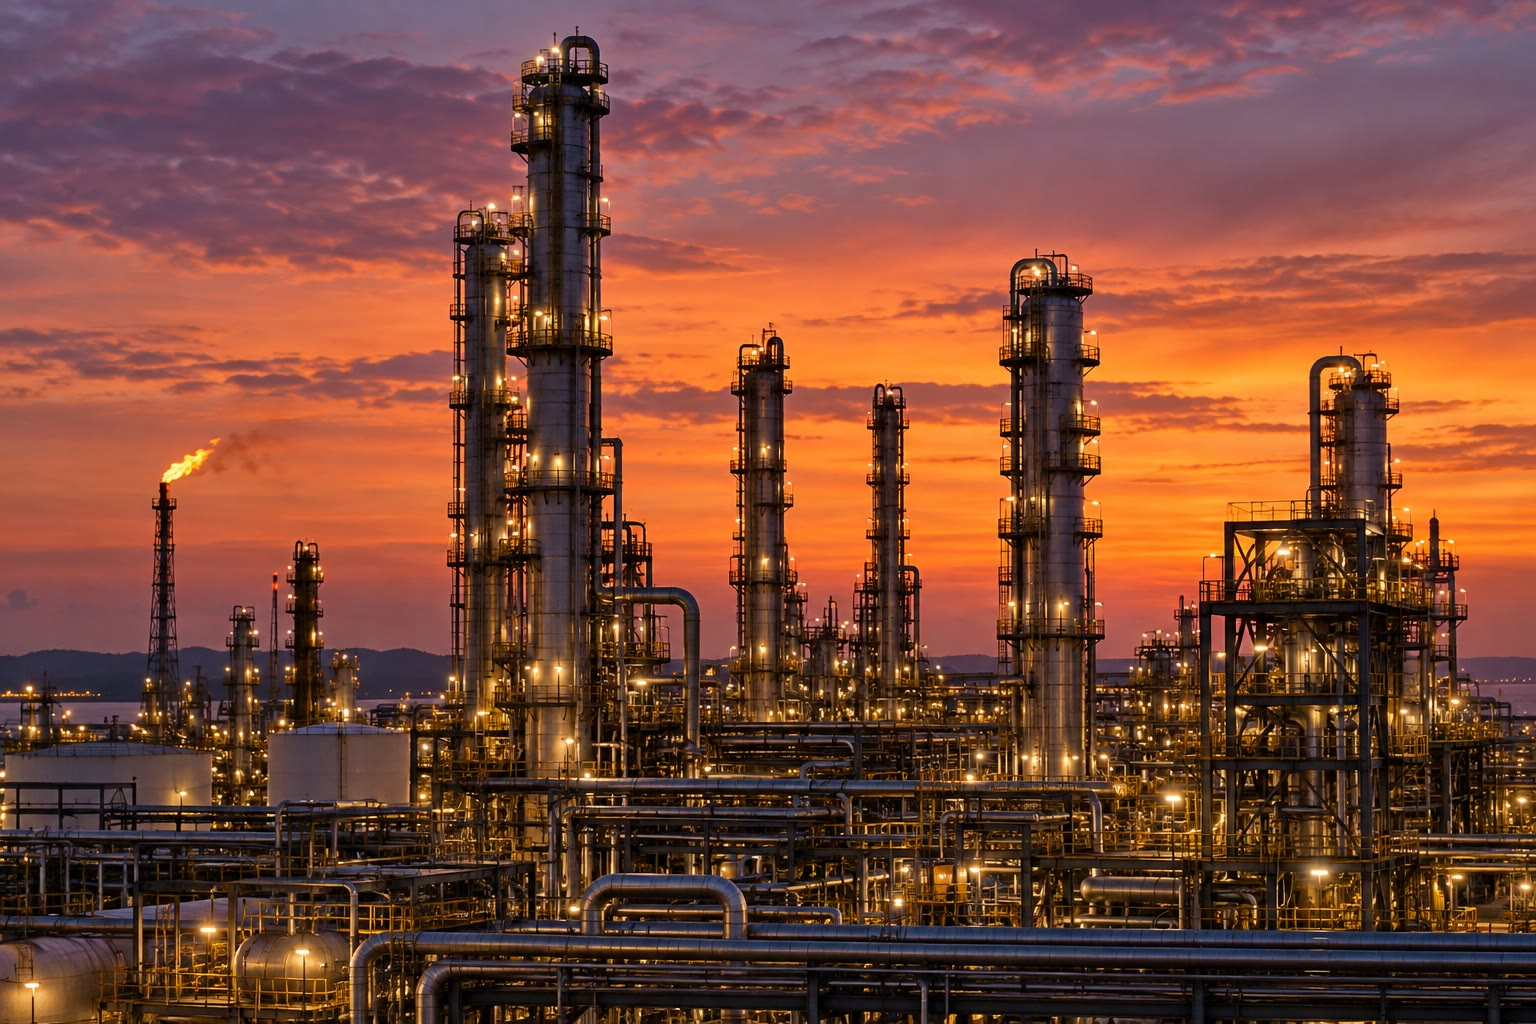
\includegraphics[width=0.52\linewidth]{images/book1/ai/g11-refinery-dusk.jpg}

{\small साँझ के समय एक रिफ़ाइनरी के \omterm{def:g10:chemical-species:distillation}{आसवन} स्तंभ।}
\end{omfigure}

\begin{safety}{\ghs[0.66cm]{GHS02}\ghs[0.66cm]{GHS04}\ghs[0.66cm]{GHS07}\ghs[0.66cm]{GHS08}\ghs[0.66cm]{GHS09}}
% ledger: ghs:butane, ghs:pentane
ब्यूटेन एक अत्यंत ज्वलनशील गैस है, जिसे दाब में रखा जाता है। पेंटेन
एक अत्यधिक ज्वलनशील द्रव है; इसकी वाष्प उनींदापन लाती है, निगलने पर यह फेफड़ों
को हानि पहुँचा सकता है और यह जलीय जीवों के लिए विषैला है। हल्के \omterm{def:g11:organic-skeletons:alkane}{ऐल्केनों} के पास
कोई लौ नहीं; धूम-हुड के नीचे काम कीजिए।
\end{safety}

\section{अभ्यास}


\begin{exercise}[$\star$]\label{exo:g11:organic-skeletons:1}
यहाँ बने \omterm{def:g7:atoms-and-molecules:molecule}{अणुओं} के \omterm{def:g11:organic-skeletons:formulas}{आण्विक सूत्र} बताइए, और बताइए कि क्या
वे \omterm{def:g11:organic-skeletons:isomer}{समावयवी} हैं:
\setchemfig{atom sep=1.6em}
\chemfig{-[:30]-[:-30]-[:30]-[:-30]-[:30]} \quad और \quad
\chemfig{-[:30](-[:90])-[:-30]-[:30]-[:-30]}।
\end{exercise}

\begin{exercise}[$\star$]\label{exo:g11:organic-skeletons:2}
नाम बताइए: \ce{CH3-CH2-CH3}; \ce{CH3-CH2-CH2-CH2-CH2-CH3};
\chemfig{CH_3-CH(-[2]CH_3)-CH_2-CH_3}।
\end{exercise}

\begin{exercise}[$\star$]\label{exo:g11:organic-skeletons:3}
प्रोपेन और 2-मेथिलप्रोपेन के \omterm{def:g11:organic-skeletons:formulas}{अर्ध-संरचना सूत्र}, और
एथेन का \omterm{def:g11:organic-skeletons:formulas}{संरचना सूत्र} लिखिए।
\end{exercise}

\begin{exercise}[$\star$]\label{exo:g11:organic-skeletons:4}
हर \omterm{def:g7:atoms-and-molecules:molecule}{अणु} के कार्बन और हाइड्रोजन \omterm{def:g7:atoms-and-molecules:atom}{परमाणु} गिनिए:
\setchemfig{atom sep=1.6em}
\chemfig{-[:30]-[:-30](-[:-90])-[:30]-[:-30]} \quad और \quad
\chemfig{*6(------)}।
\end{exercise}

\begin{exercise}[$\star$]\label{exo:g11:organic-skeletons:5}
8 कार्बन \omterm{def:g7:atoms-and-molecules:atom}{परमाणुओं} वाले \omterm{def:g11:organic-skeletons:alkane}{ऐल्केन} का \omterm{def:g11:organic-skeletons:formulas}{आण्विक सूत्र}, और 20 हाइड्रोजन \omterm{def:g7:atoms-and-molecules:atom}{परमाणुओं} वाले
\omterm{def:g11:organic-skeletons:alkane}{ऐल्केन} के कार्बन \omterm{def:g7:atoms-and-molecules:atom}{परमाणुओं} की संख्या बताइए।
\end{exercise}

\begin{exercise}[$\star\star$]\label{exo:g11:organic-skeletons:6}
3-मेथिलहेक्सेन, 2,2-डाइमेथिलब्यूटेन और 3-एथिलपेंटेन के \omterm{def:g11:organic-skeletons:formulas}{कंकाल सूत्र}
बनाइए, और उनके \omterm{def:g11:organic-skeletons:formulas}{आण्विक सूत्र} बताइए।
\end{exercise}

\begin{exercise}[$\star\star$]\label{exo:g11:organic-skeletons:7}
\ce{C5H12} के तीनों \omterm{def:g11:organic-skeletons:isomer}{समावयवी} बनाइए और उनके नाम बताइए।
\end{exercise}

\begin{exercise}[$\star\star$]\label{exo:g11:organic-skeletons:8}
ये नाम ग़लत हैं। हर \omterm{def:g7:atoms-and-molecules:molecule}{अणु} बनाइए और उसका सही नाम बताइए:
2-एथिलब्यूटेन; 4-मेथिलपेंटेन; 1-मेथिलब्यूटेन।
\end{exercise}

\begin{exercise}[$\star\star$]\label{exo:g11:organic-skeletons:9}
\ce{C5H12} के \omterm{def:g11:organic-skeletons:isomer}{समावयवियों} वाले चित्र की मदद से उन्हें क्वथन ताप के अनुसार क्रम
दीजिए और क्रम समझाइए।
\end{exercise}

\begin{exercise}[$\star\star$]\label{exo:g11:organic-skeletons:10}
साइक्लोहेक्सेन \ce{C6H12} है और हेक्सेन \ce{C6H14}। दो कम हाइड्रोजन \omterm{def:g7:atoms-and-molecules:atom}{परमाणुओं}
को समझाइए। क्या ये दोनों यौगिक \omterm{def:g11:organic-skeletons:isomer}{समावयवी} हैं? क्या साइक्लोहेक्सेन एक
\omterm{def:g11:organic-skeletons:alkane}{ऐल्केन} है?
\end{exercise}

\begin{exercise}[$\star\star$]\label{exo:g11:organic-skeletons:11}
प्रोपेन, ब्यूटेन, 2-मेथिलप्रोपेन और साइक्लोब्यूटेन (\ce{C4H8}, चार कार्बन \omterm{def:g7:atoms-and-molecules:atom}{परमाणुओं}
का एक वलय) में से कौन एक-दूसरे के \omterm{def:g11:organic-skeletons:isomer}{समावयवी} हैं?
\end{exercise}

\begin{exercise}[$\star\star\star$]\label{exo:g11:organic-skeletons:12}
\ce{C6H14} के पाँचों \omterm{def:g11:organic-skeletons:isomer}{समावयवी} बनाइए और उनके नाम बताइए।
\end{exercise}

\begin{exercise}[$\star\star\star$]\label{exo:g11:organic-skeletons:13}
किसी रैखिक \omterm{def:g11:organic-skeletons:alkane}{ऐल्केन} को एक लंबी टेढ़ी-मेढ़ी रेखा और बहुत शाखित \omterm{def:g11:organic-skeletons:alkane}{ऐल्केन} को एक गेंद
मानिए। इस चित्र की मदद से समझाइए कि शाखन \omterm{def:g11:organic-skeletons:isomer}{समावयवियों} के क्वथन
ताप को क्यों घटाता है।
\end{exercise}

\begin{exercise}[$\star\star\star$]\label{exo:g11:organic-skeletons:14}
इस \omterm{def:g11:organic-skeletons:alkane}{ऐल्केन} का नाम बताइए:
\begin{center}
\chemfig{CH_3-CH(-[2]CH_3)-CH_2-C(-[2]CH_3)(-[6]CH_3)-CH_2-CH_3}
\end{center}
\end{exercise}

\begin{exercise}[$\star\star\star$]\label{exo:g11:organic-skeletons:15}
पेट्रोल का संदर्भ यौगिक, ``आइसो-ऑक्टेन'',
2,2,4-ट्राइमेथिलपेंटेन है। उसका \omterm{def:g11:organic-skeletons:formulas}{कंकाल सूत्र} बनाइए, जाँचिए कि वह ऑक्टेन का
\omterm{def:g11:organic-skeletons:isomer}{समावयवी} है, और उसका \omterm{def:g11:organic-skeletons:formulas}{अर्ध-संरचना सूत्र} लिखिए।
\end{exercise}

\section{समस्या: लाइटर की गैस}

\begin{problem}[{सप्ताहांत समस्या --- सूत्र
\ce{C7H16} वाले कितने अलग-अलग \omterm{def:g11:organic-skeletons:alkane}{ऐल्केन} हैं?}]
\label{pb:g11:organic-skeletons:1}
% ledger: bp:C3H8, bp:C4H10, bp:isobutane
लाइटर में ब्यूटेन होती है; सर्दियों के कैंपिंग कारतूस में ऐसा \omterm{def:g6:pure-substances-and-mixtures:mixture}{मिश्रण} होता है जिसमें
प्रोपेन या 2-मेथिलप्रोपेन अधिक हो। ब्यूटेन लगभग
\qty{0}{\celsius} पर उबलती है, 2-मेथिलप्रोपेन \qty{-11.7}{\celsius} पर और प्रोपेन
\qty{-42}{\celsius} पर।

\medskip
\noindent\textbf{भाग I --- एक सूत्र वाली दो गैसें।}
\begin{enumerate}
  \item ब्यूटेन का \omterm{def:g11:organic-skeletons:formulas}{आण्विक सूत्र} बताइए, और जाँचिए कि वह \omterm{def:g11:organic-skeletons:alkane}{ऐल्केनों} के
        सामान्य सूत्र में बैठता है।
  \item उसका \omterm{def:g11:organic-skeletons:formulas}{संरचना सूत्र} बनाइए।
  \item उसके अर्ध-संरचना और \omterm{def:g11:organic-skeletons:formulas}{कंकाल सूत्र} लिखिए।
  \item 2-मेथिलप्रोपेन को इन्हीं तीन तरह से बनाइए। उसका \omterm{def:g11:organic-skeletons:formulas}{आण्विक सूत्र}
        वही क्यों है?
  \item क्या ब्यूटेन और 2-मेथिलप्रोपेन \omterm{def:g11:organic-skeletons:isomer}{समावयवी} हैं? किस प्रकार के?
\end{enumerate}

\medskip
\noindent\textbf{भाग II --- ठंड में।}
\begin{enumerate}[resume]
  \item \qty{20}{\celsius} और सामान्य दाब पर तीनों में से कौन-सी
        गैसें हैं?
  \item एक खुला लाइटर \qty{-5}{\celsius} पर बाहर इस्तेमाल किया जाता है। वह
        कमज़ोर लौ क्यों देता है?
  \item सर्दियों के कारतूसों में प्रोपेन या 2-मेथिलप्रोपेन अधिक क्यों होती है?
  \item समझाइए कि 2-मेथिलप्रोपेन ब्यूटेन से कम ताप पर क्यों उबलती है।
  \item प्रोपेन का कोई \omterm{def:g11:organic-skeletons:isomer}{समावयवी} क्यों नहीं है?
\end{enumerate}

\medskip
\noindent\textbf{भाग III --- नाम रखना और गिनना।}
\begin{enumerate}[resume]
  \item \chemfig{CH_3-CH(-[2]CH_3)-CH_2-CH_3} का नाम बताइए।
  \item उसी \omterm{def:g7:atoms-and-molecules:molecule}{अणु} के लिए ``3-मेथिलब्यूटेन'' नाम ग़लत क्यों है?
  \item सूत्रों \ce{C4H10},
        \ce{C5H12} और \ce{C6H14} वाले कितने \omterm{def:g11:organic-skeletons:alkane}{ऐल्केन} \omterm{def:g11:organic-skeletons:isomer}{समावयवी} हैं?
\end{enumerate}

\medskip
\noindent\textbf{भाग IV --- \ce{C7H16} के \omterm{def:g11:organic-skeletons:isomer}{समावयवी}।}
\begin{enumerate}[resume]
  \item रैखिक \omterm{def:g11:organic-skeletons:isomer}{समावयवी} बनाइए और उसका नाम बताइए।
  \item वे \omterm{def:g11:organic-skeletons:isomer}{समावयवी} बनाइए और उनके नाम बताइए जिनकी सबसे लंबी श्रृंखला में छह कार्बन
        \omterm{def:g7:atoms-and-molecules:atom}{परमाणु} हैं। ``4-मेथिलहेक्सेन'' क्यों नहीं होता?
  \item वे \omterm{def:g11:organic-skeletons:isomer}{समावयवी} बनाइए और उनके नाम बताइए जिनकी सबसे लंबी श्रृंखला में पाँच कार्बन
        \omterm{def:g7:atoms-and-molecules:atom}{परमाणु} और दो मेथिल समूह हैं।
  \item क्या पाँच-कार्बन श्रृंखला और एक एथिल समूह वाला कोई \omterm{def:g11:organic-skeletons:isomer}{समावयवी} है?
        एथिल समूह केवल कार्बन 3 पर ही क्यों हो सकता है?
  \item वह \omterm{def:g11:organic-skeletons:isomer}{समावयवी} बनाइए और उसका नाम बताइए जिसकी सबसे लंबी श्रृंखला में चार कार्बन
        \omterm{def:g7:atoms-and-molecules:atom}{परमाणु} हैं।
  \item मिले सभी \omterm{def:g11:organic-skeletons:isomer}{समावयवी} गिनिए।
  \item अंतिम उत्तर बताइए: हेप्टेन के, स्वयं उसे मिलाकर, कितने \omterm{def:g11:organic-skeletons:isomer}{संरचनात्मक
        समावयवी} हैं?
\end{enumerate}
\end{problem}
